\documentclass[aspectratio=169]{beamer}

\usetheme{simple}

\usepackage{lmodern}
\usepackage[scale=2]{ccicons}
\centering

% TODO: 
%   position adjustement
%   change colours
%       

% Watermark background (simple theme)


\setwatermark{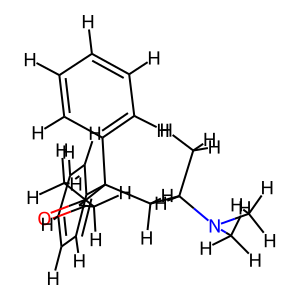
\includegraphics[height=8cm]{img/Methadone_Overlay.png}}


\title{Ligands and Receptors: A Love Story}
\subtitle{Binding Affinities Between Opioids and the $\mu$-opioid Receptor}
\date{\today}
\author{Joshua Stoneburner}
\institute{\url{https://github.com/JoshuaKSt}}

\begin{document}

\maketitle

\setwatermark{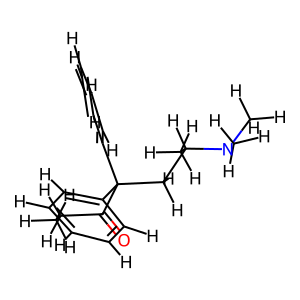
\includegraphics[height=8cm]{img/MethadoneMOL_Overlay.png}}
\begin{frame}{Research Goal}

    \begin{columns}
        \column{.5\textwidth}
            \begin{itemize}
            \item Direction.
            \item Understand opioid receptors.
            \item Create a molecule. 
            \item Simulate its interaction with the $\mu$-opioid receptor and compare.
      \end{itemize}
    \end{columns}
    \end{frame}



\setwatermark{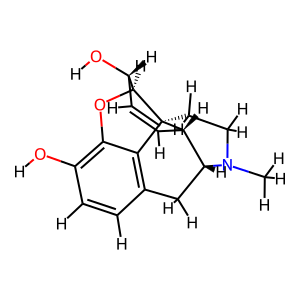
\includegraphics[height=8cm]{img/MorphineMOL_Overlay.png}}
\begin{frame}{Molecule Creation and Optimization Method}
    \begin{columns}
        \column{.5\textwidth}
            \begin{itemize}
            \item Generating the molecule using RDKit.
            \item Optimization of drug bank molecules.
      \end{itemize}
    \end{columns}
\end{frame}

\setwatermark{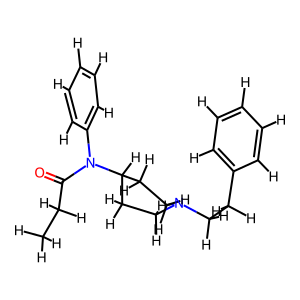
\includegraphics[height=8cm]{img/FentanylSDF_Overlay.png}}
\begin{frame}{Conformer Energy Graphs}
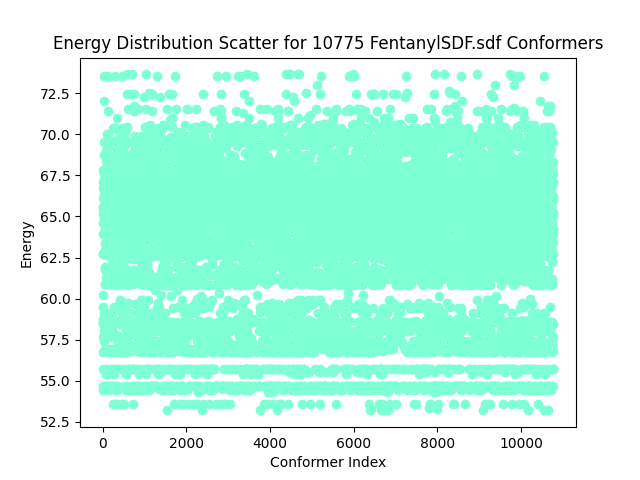
\includegraphics[width=10cm]{img/Graphs/FentanylSDF_Energy_Scatter.png}
\end{frame}
\setwatermark{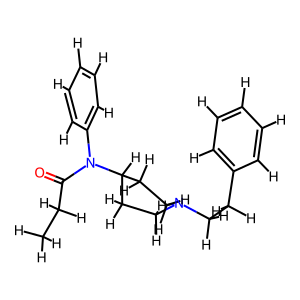
\includegraphics[width=8cm]{img/FentanylSDF_Overlay.png}}
\begin{frame}{Conformer Energy Graphs}
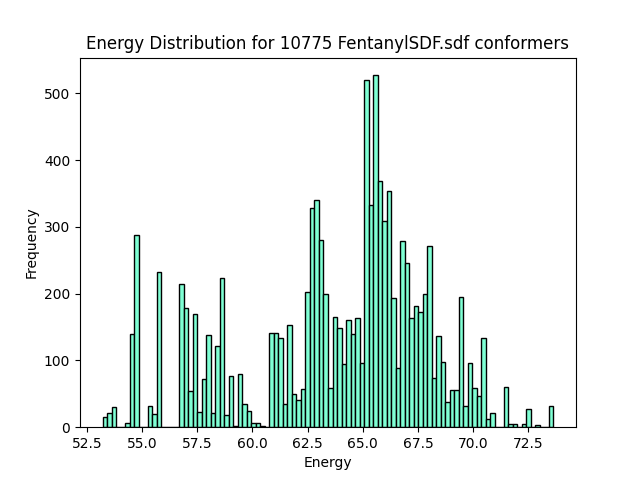
\includegraphics[width=10cm]{img/Graphs/FentanylSDF_Energy_Histogram.png}
\end{frame}

\setwatermark{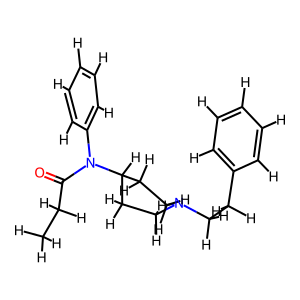
\includegraphics[height=8cm]{img/FentanylSDF_Overlay.png}}
\begin{frame}{Conformer Energy Graphs}
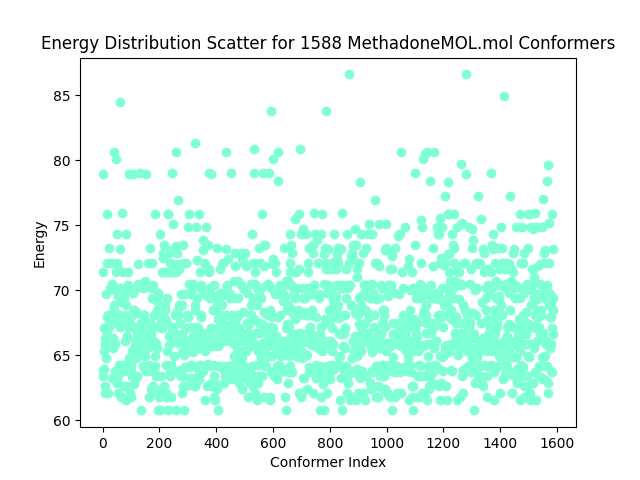
\includegraphics[width=10cm]{img/Graphs/MethadoneMOL_Energy_Scatter.png}
\end{frame}
\setwatermark{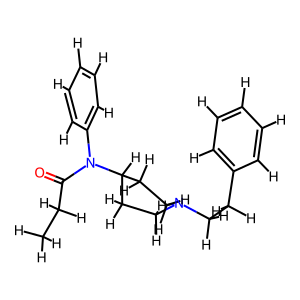
\includegraphics[width=8cm]{img/FentanylSDF_Overlay.png}}
\begin{frame}{Conformer Energy Graphs}
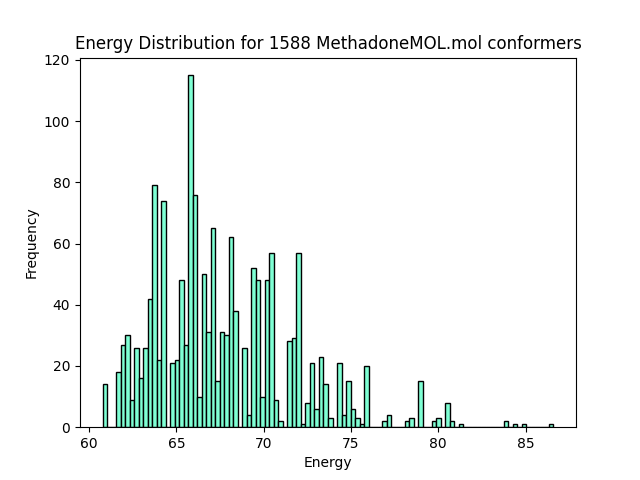
\includegraphics[width=10cm]{img/Graphs/MethadoneMOL_Energy_Histogram.png}
\end{frame}

\setwatermark{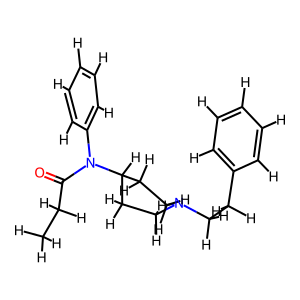
\includegraphics[height=8cm]{img/FentanylSDF_Overlay.png}}
\begin{frame}{Conformer Energy Graphs}
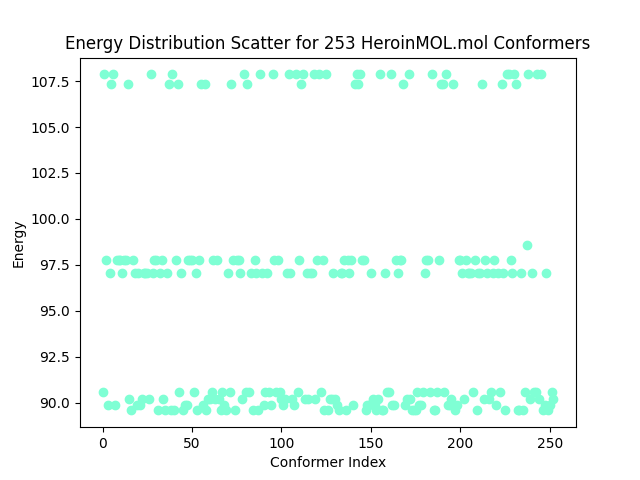
\includegraphics[width=10cm]{img/Graphs/HeroinMOL_Energy_Scatter.png}
\end{frame}
\setwatermark{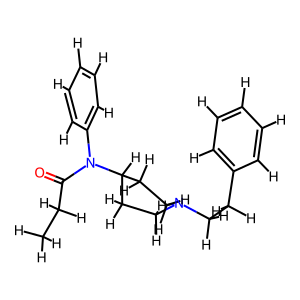
\includegraphics[width=8cm]{img/FentanylSDF_Overlay.png}}
\begin{frame}{Conformer Energy Graphs}
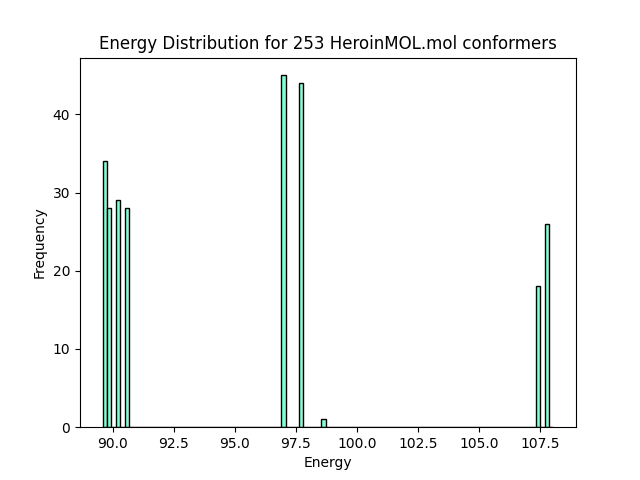
\includegraphics[width=10cm]{img/Graphs/HeroinMOL_Energy_Histogram.png}
\end{frame}

\setwatermark{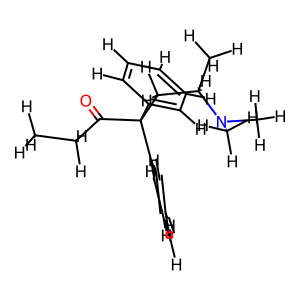
\includegraphics[height=8cm]{img/methadone_angled_overlay.png}}
\begin{frame}{Experiment Setup}
    \begin{columns}
        \column{.5\textwidth}
            \begin{itemize}
            \item Receptor finding and pruning.
            \item Simulate!
      \end{itemize}
    \end{columns}
\end{frame}

\setwatermark{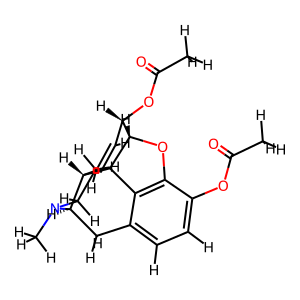
\includegraphics[height=8cm]{img/HeroinMOL_Overlay.png}}

\begin{frame}{What are: "Binding Affinities"?}
  \framesubtitle{}

\begin{flushleft}
 \texttt They are:
\end{flushleft}

  \begin{columns}
    \column{.5\textwidth}
      \begin{itemize}
        \item How tightly bound an interaction is \\(i.e. a ligand and protein) 
        \item Often referred to as the free energy of binding ($\Delta G$)
        \item Used in drug optimization, computations of biological systems etc.
      \end{itemize}

    \column{.5\textwidth}
      \begin{block}{Simple terms in context of my research:}
         The total energy decrease when a ligand binds to a receptor
      \end{block}
  \end{columns}
  
\end{frame}

\setwatermark{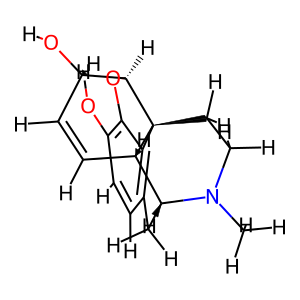
\includegraphics[height=8cm]{img/MorphineSDF_Overlay.png}}
\begin{frame}{Briefing}
    \begin{columns}
        \column{.5\textwidth}
            \begin{itemize}
                \item $\mu$-opioid Receptors
                \begin{itemize} \scriptsize
                    \item 6DDF (Human, Mouse, Removed DAMGO)
                    \item 8E0G (Mouse, Llama, Removed BU72)
                    \item 8K9K (Human, Removed DAMGO)
                \end{itemize}
                \item Ligands
                \begin{itemize} \footnotesize
                    \item Heroin
                    \item Morphine
                    \item Fentanyl
                    \item Methadone
                    \item Carfentanil
                    \item BU72
                \end{itemize}
                \item .SDF and .MOL
                \begin{itemize} \footnotesize
                    \item Structure Data Files
                \end{itemize}
            \end{itemize}
        \end{columns}
        
\end{frame}

\setwatermark{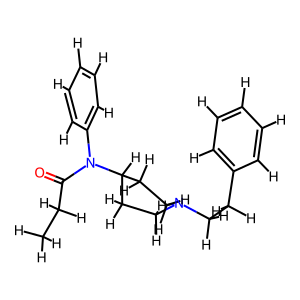
\includegraphics[width=1cm]{img/FentanylSDF_Overlay.png}}
\begin{frame}{Heroin 6DDF Docking Output}
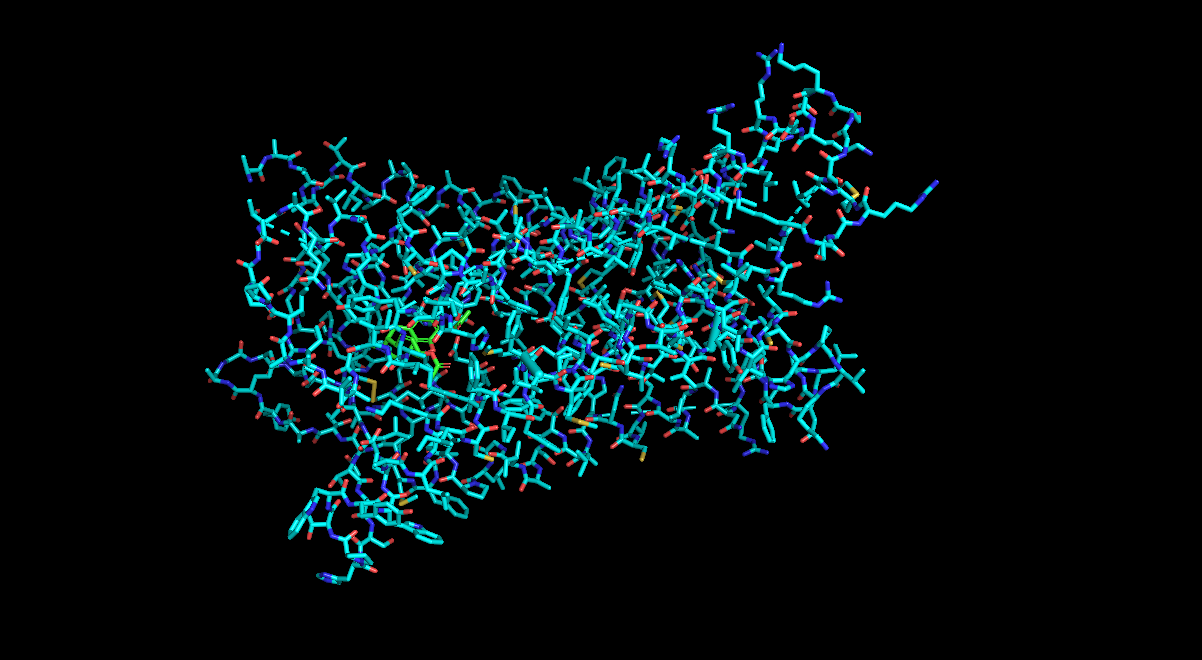
\includegraphics[width=12cm]{img/Graphs/6ddfSide.png}
\end{frame}
\begin{frame}{Heroin 8E0G Docking Output}
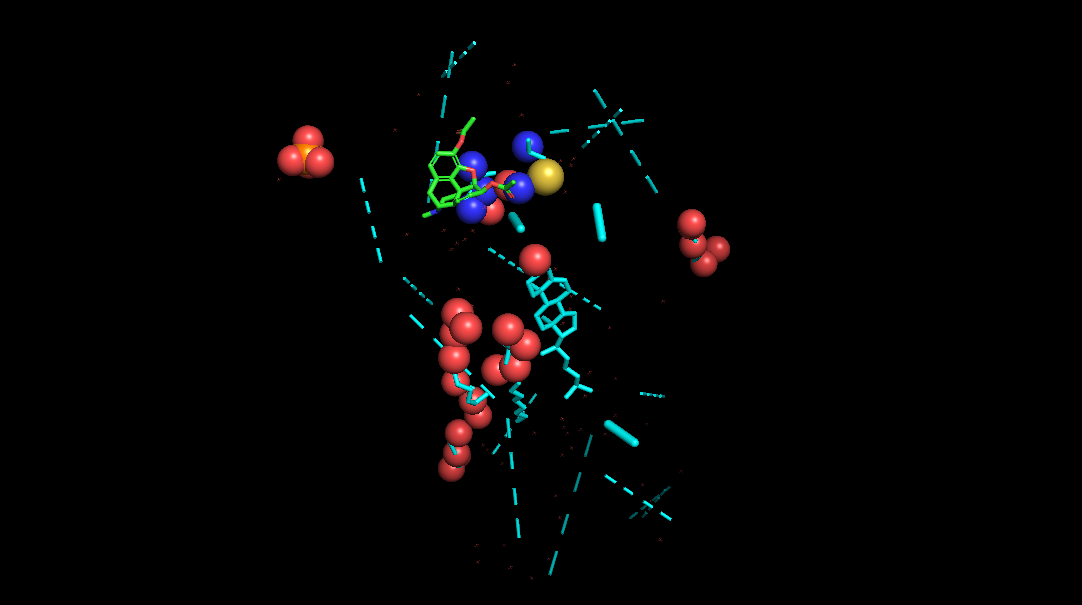
\includegraphics[width=12cm]{img/Graphs/8e0gTransparent.png}
\end{frame}
\begin{frame}{Heroin 8E0G Docking Output}
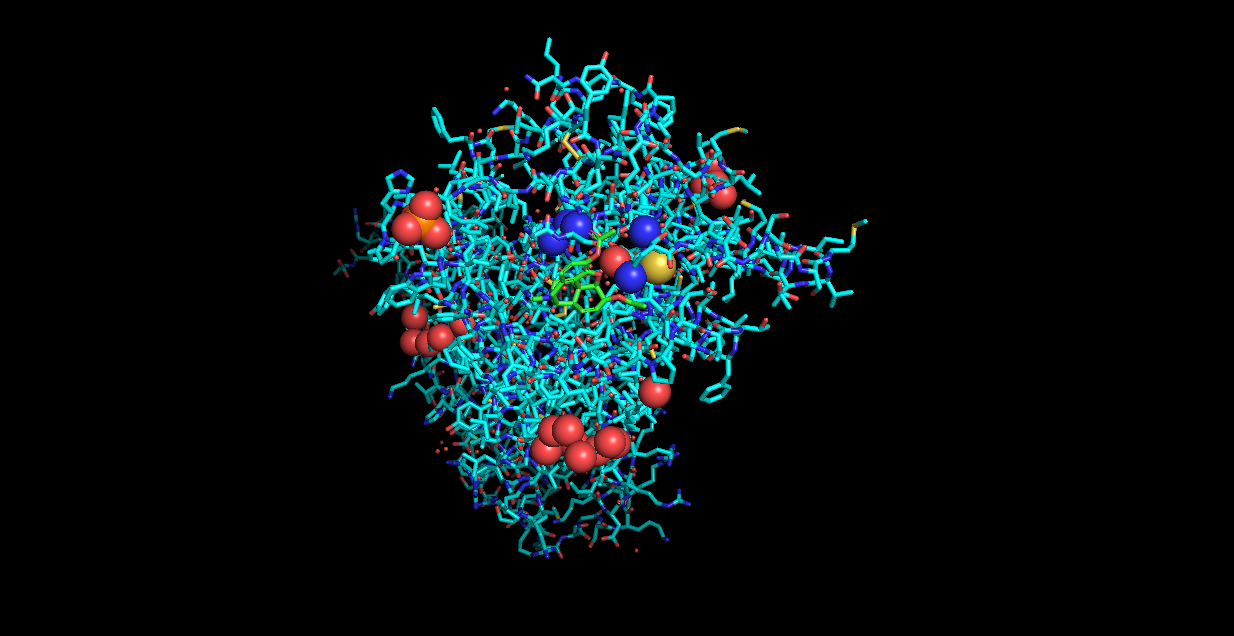
\includegraphics[width=12cm]{img/Graphs/8e0gFull.png}
\end{frame}
\begin{frame}{Affinity Graphs}
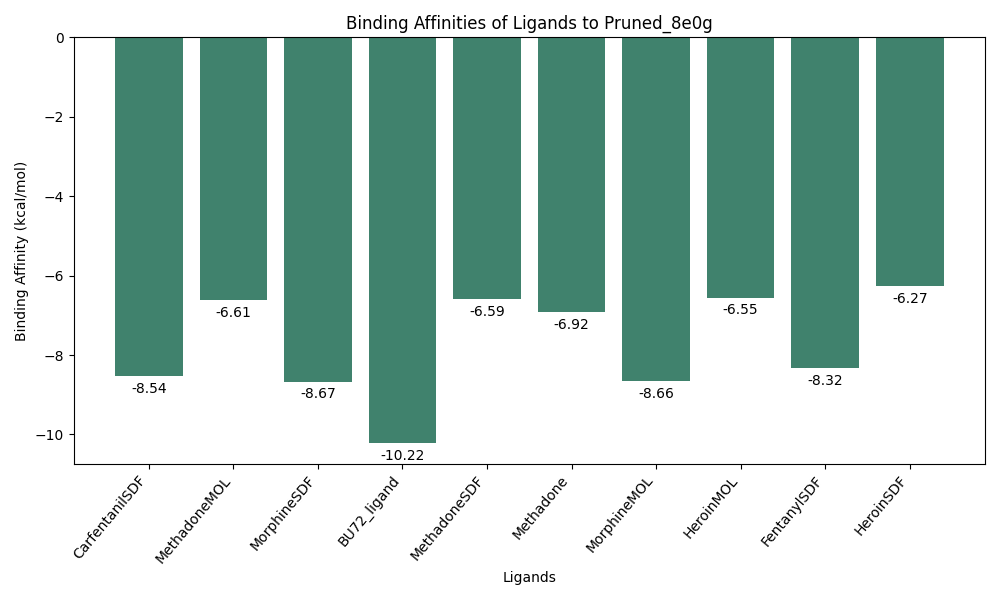
\includegraphics[width=12cm]{img/Graphs/Pruned_8e0g_affinities.png}
\end{frame}

\begin{frame}{Affinity Graphs}
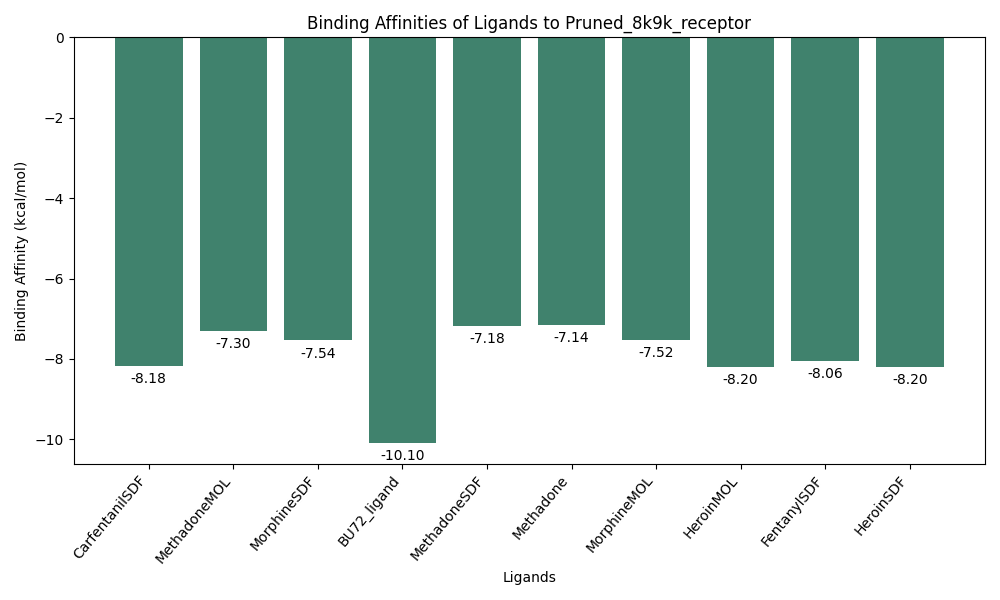
\includegraphics[width=12cm]{img/Graphs/Pruned_8k9k_receptor_affinities.png}
\end{frame}
\begin{frame}{Affinity Graphs}
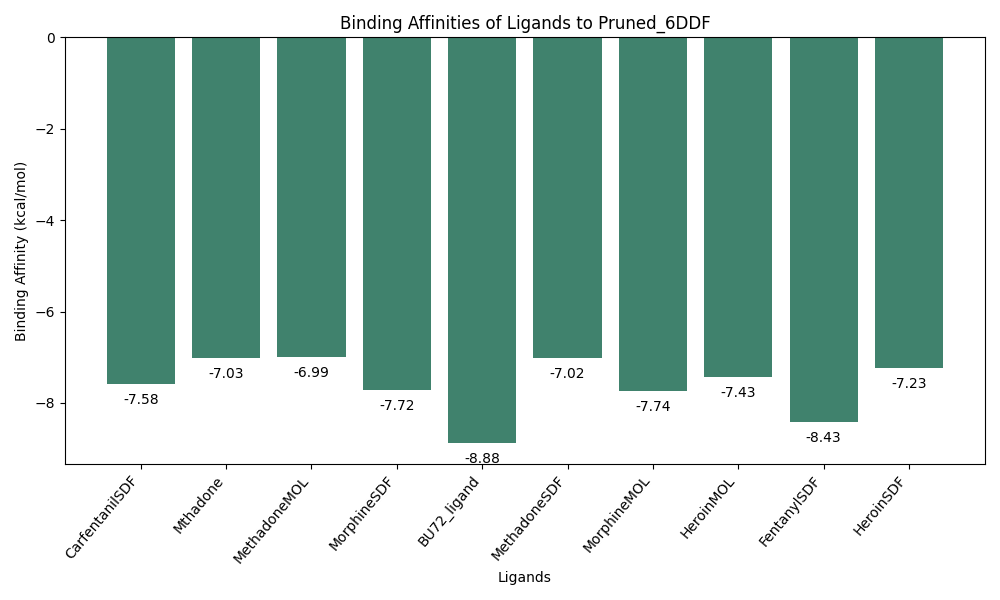
\includegraphics[width=12cm]{img/Graphs/Pruned_6DDF_affinities.png}
\end{frame}

\setwatermark{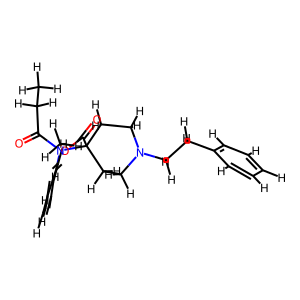
\includegraphics[height=8cm]{img/CarfentanilSDF_Overlay.png}}
\begin{frame}{Analysis}
    \begin{columns}
        \column{.5\textwidth} \footnotesize
            \begin{itemize}
                \item BU72 Consistently had the strongest binding.
                \item Fentanyl and Carfentanil consistently showed strong binding.
                \item Morphine was stronger bound to a higher quality model.
                \item The gap in affinity lessened when the structure was lower quality.
                \item Heroin and Methadone varied greatly across structure and file format.
            
      \end{itemize}
    \end{columns}
\end{frame}

\setwatermark{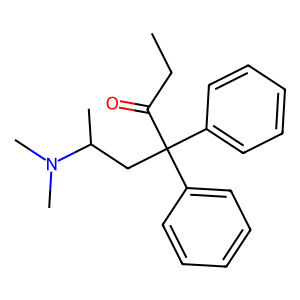
\includegraphics[height=8cm]{img/Graphs/Methadone_Overlay.png}}
\begin{frame}{Thank You!}
\end{frame}

\end{document}